%===================================== CHAP 2 =================================

\chapter{Literature Review and Background} \label{cap_2}

\section{Related work}

\subsection{Semi-structured text}
When extracting information from a textual document, it is important to know how structured the text is. There are two extremes that the document most likely falls between, \textit{structured data} and \textit{free text}  \cite{semi-struc-text}. Structured data is using data models for organizing and standardizing data elements, also including their relations. The other extreme, free text, is unstructured as a newspaper article. Wikipedia's articles exists somewhere between these two extremes. We define a Wikipedia article as semi-structured text. We define it as semi-structured because the articles from Wikipedia are created from a comprehensive markup language. The articles are also stored in the form of this markup language. Because of that we can extract the information from the article's markup and not from the page presented to the readers at the Wikipedia page. 

The fact that the articles are semi-structured is an advantage when extracting information. In Wikipedia's case all sections has a header, which lets us not only know the subject of the sections content, but it also shows its position in the hierarchy of all the article's sections. These added tags to the text makes it self-describing, making it possible for us to find the semantics of the text easier. It also defines the hierarchy of different parts in the text, like sections, records or fields. In free text subtle inferences are required based on grammar to create domain objects, which in turn will describe the semantics of the text. 

\subsection{Wikimedia} \label{wikimedia}
Wikimedia \cite{wikimedia} is an organization that supports and manages many different knowledge projects. Their goal is to make free knowledge accessible anywhere and on any platform. Their income comes primarily from donations. They do not make us of ads, because they believe it could jeopardize their reliability as a neutral source of information.

Wikimedia is mostly known for Wikipedia \cite{wikipedia}. Wikipedia is the largest collection of free, collaborative knowledge that exists. Wikipedia can be found in over 290 languages and across those, contains more than 35 million articles. Our project will make use of the English Wikipedia, which contains more than 5 million articles. Wikipedia uses a  software called MediaWiki \cite{mediawiki}. It is a server side software used for hosting wiki sites. Many of the wiki sites under the Wikimedia umbrella makes use of MediaWiki. A part of the MediaWiki software is the markup language used for writing articles. This markup, written by contributors, will then later be translated into HTML when displayed for users in their web browser. This markup is used to create elements such as tables, equations, lists and links. Wikimedia regularly backs up Wikipedia and makes it publicly available as a large XML file. The XML file provides access to the raw data of articles, which is the article's metadata and the content of the article in MediaWiki markup. The metadata gives access to useful information such as id, title and revision. The revision data includes author and timestamp. The metadata also let us determine if the article contains content itself or if it just redirects to another article.

Public access to this information gives a lot of opportunities. Alberto Montero-Asenjo and Carlos A. Iglesias used a XML dump from the Spanish Wikipedia for language research \cite{lr-wiki}. They created a piece of software that processes the raw source data from the XML dump. It starts by converting the Wiki markup into plain text and then use further operations on the plain text to make the end result of useful data. While they use the raw data for language research, we need to extract more information from the source data, by looking at the markup in order to extract the semi-structured text. Section headers, references, code tags and categories, are examples of extra information the markup makes available. 
To gain the extra information made available by the markup, the syntax and the semantics behind it has to be interpreted, instead of filtering it away.
How to interpret the semantics that the markup reveals, has been touched on and discussed in section \ref{sec_tdm} and a couple of articles \cite{text-cat} \cite{wlm}. There is though a surprisingly lack of work about the interpretation of the markups syntax itself. Because of this, we have had to build this from the ground up, with help from a Wikipedia page created for assisting people writing the articles\footnote{\url{https://en.wikipedia.org/wiki/Help:Wiki_markup}}. You can read more about our work on this issue in sections \ref{cap_3} and \ref{cap_4}.

\subsection{Text data mining} \label{sec_tdm}
This projects aims at extracting example sections from articles on Wikipedia and then find relations among them. Therefor this project is related to two research fields. One of the research fields is information retrieval (IR), which mainly is about helping users finding documents of their needs \cite{irbook}. The other research field is text data mining (TDM), where the goal is to discover useful information from textual data. Hearst discusses methods that can help us find and extract example sections from Wikipedia in her work, Untangling text data mining \cite{untanglingTDM}. She explains how to find patterns across data sets and finding relevant information among a collection of mostly irrelevant data. She achieves this by focusing on a mixture between computationally-driven and user-guided analysis, rather than a fully artificial intelligent text analysis.


To be able to discover relevant data from the Wikipedia articles, Wikimedia's markup language has to be interpreted.  To interpret the articles, we will focus on the structure that we can derive from its markup. The articles' structure mainly consists of section headers followed by the textual content of the section. There is also other information that can be extracted. To find relations between articles we would also need to look at the semantics from this information, such as lists, categories and references, amongst others. YAWN\footnote{Yet Another Wikipedia Annotation project}, is a project that created an XML version of Wikipedia with focus on semantic information \cite{yawn}. The XML corpus produced by YAWN is general for the whole Wikipedia and the entire article collection. Our project focuses only on the articles that are relevant for educational purpose and comprising examples to explain its content. Although YAWN does more than what is needed for our purpose, key concepts and techniques for exploiting the Wiki markup, can be derived and used for classifying examples in this project. The most interesting for this project is how it finds semantic annotations for Wikipedia pages. In order to do so, it uses a combination of exploiting information about categories assigned to articles and deriving information from the structure of an article.

Making heavy use of categories is a straight forward method to discover relations between examples. However making use of other information in the articles, would further increase the accuracy of the relations discovered. Internal links between articles is another way we can mine data about relations between articles. Links also force us to consider the difference between a link going into an article, and a link going from one. Evgeniy Gabrilovich and Shaul Markovitch used Wikipedia as a knowledge repository in an effort to enhance text categorization  \cite{text-cat}. They made use of links and their sometimes differing \textit{anchor texts}\footnote{Display text of the link} to improve their text categorization. A concept they took advantage of were that different anchor texts for the same link can indicate different contexts.  They also looked at number of incoming links to an article. In contrast, our project aims to look deeper into the relationships between articles. We aim to utilize the information about how one article links to another and if that makes them related. David Milne and Ian H. Witten look more into this connection between articles in their approach,  Wikipedia Link-based Measure (WLM) \cite{wlm}. Here they used mainly two methods to measure the relatedness between two articles, based on links. The first one is an approach similar to TF-IDF\footnote{term frequency inverse document frequency}, a information retrieval algorithm explained in section \ref{tf/idf}, where they count links instead of terms. They then create vectors according to the vector space model and then finds the similarity of two articles based on the angle of their vectors. The second method they use are modeled after the Normalized Google Distance  \cite{gsd}. Here the simply assumes that two articles containing the same link indicates relatedness. On the other hand, if one article contain a specific link which the other do not, it indicates the opposite.

\subsection{SMILA} \label{smila}

\begin{figure}[h]
\caption{An overall overview of the SMILA architecture}
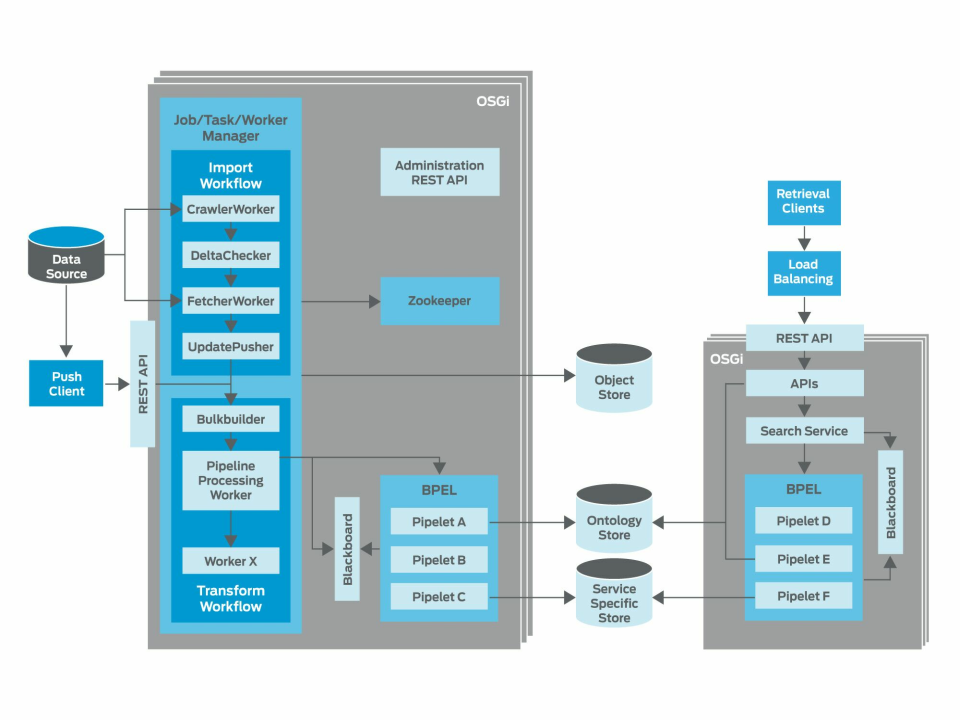
\includegraphics[width=\textwidth]{SMILA_Architecture}
\end{figure}

%%fix sånn abbrevation for SMILA

%%når jeg snakker om mine erfaringer med smila gjør jeg det i implementation.

In the early stages of our project, an existing tool called SMILA \cite{smila} was explored. SMILA is a system with its first release in 2010, it is used to search and access unstructured information. SMILA crawls the web to extract information and then stores the information in an index. It has a REST API to control the system and for searching the index. The SMILA architecture is also based on the pipeline architecture containing the following processes; jobs, crawling, storage, indexing and querying. Since 2010, 6 new versions has been released adding more features to SMILA. With SMILA being very complex, it gains asynchronicity as its biggest benefit from the pipeline architecture. The SMILA pipeline also allows custom made pipelets to be inserted into the pipeline. A pipelet is a sub process inside a pipeline. By creating pipelets, the behaviour of SMILA could be tailored into extracting relevant information from Wikipedia.

The releases for SMILA has been dwindling the last three years with only 1 release in 2015. If you add that to the fact that all the different features of SMILA makes it very complex, the usability and stability suffers. This was experienced during testing of the program during this project.
Nevertheless the utility that the SMILA system offers could be taken advantage of in this project. Either by utilizing SMILA itself, or look at how SMILA retrieves data from the web, processes it and produces a data set as a result.


\section{Techniques / Methodology}

\subsection{Pipeline} \label{pipeline}

A software pipeline is a chain of processes where the output of one process is fed as input into another. Arrange these processes correctly and the result is a pipeline. A software pipeline is actually a design pattern, where it is better known as \textit{pipes and filters} \cite{pipes-and-filters}. The two big advantages of a software pipeline is modularity and parallelity \cite{dart}. The reason for parallelity is that the data can be spread across several processes. This means that the data can be processed in different instances of the program. Another case is more like a conveyor belt, where data is propagated through the pipeline. So while some of the data are being inputted into the first stages, another part of the data is finalized at the end. The other advantage, modularity, simply means that it is easy to replace a part of the pipeline. The reason for this is that the sub processes are \textit{loosely coupled}, so changing one part of the system will not affect the rest in any way.

The first mentioned advantage, parallelity, is not used to a significant extent in this project. This is mostly because performance has not been an important quality attribute. Instead the focus has been more on functionality. For this reason the modularity part has been very valuable. It has allowed different parts of the system to be easily replaced or altered in conjunction with the changes of the requirements.


\subsection{TF-IDF} \label{tf/idf}
TF-IDF is a statistical measure which evaluates how important a word is to a document based on the document itself and the collection it is part of. Based on this it is possible to decide how likely it is for the document to be relevant. TF-IDF is used as the standard similarity measure in ElasticSearch, see section \ref{elasticsearch}.

TF-IDF can be divided into two parts, \textit{term frequency} and \textit{inverse document frequency}. \textit{Term frequency} is how often a term appears in a document. The more instances the document has of the word, the higher is the chance of the document being relevant. \textit{Inverse document frequency} looks at how often a term appears in the whole collection of documents. The more often a term appears, the less relevant is the term. This means the common terms will have less weight than rare ones, when calculating the likelihood of the documents relevance.

To calculate the similarity the formula needs a term \(t\), a document \(d\) and a document collection \(D\). TF-IDF is then calculated as
\[tfidf(t, d, D) = tf(t, d)  \cdot idf(t, D)\]
Both the term frequency and the inverse document frequency can use various ways to determine the exact values, following is two simple variants: 
\[tf(t, d) = f_{t,d}\] 
\[idf(t, D) = \frac{|D|}{ |\{d \in D: t \in d\}| }\]
Here \(f_{t,d}\) denotes the raw term frequency of \(t\) and \( |\{d \in D: t \in d\}| \) is how many documents \(t\) appears in. A high measure weight for the term will then be given by it having a high frequency in the document, but a low frequency in the overall collection.



\cleardoublepage